%%% File-Information {{{
%%% Filename: template_bericht.tex
%%% Purpose: lab report, technical report, project report
%%% Time-stamp: <2004-06-30 18:19:32 mp>
%%% Authors: The LaTeX@TUG-Team [http://latex.tugraz.at/]:
%%%          Karl Voit (vk), Michael Prokop (mp), Stefan Sollerer (ss)
%%% History:
%%%   20050914 (ss) correction of "backref=true" to "backref" due to hyperref documentation
%%%   20040630 (mp) added comments to foldmethod at end of file
%%%   20040625 (vk,ss) initial version
%%%
%%% Notes:
%%%
%%%
%%%
%%% }}}
%%%%%%%%%%%%%%%%%%%%%%%%%%%%%%%%%%%%%%%%%%%%%%%%%%%%%%%%%%%%%%%%%%%%%%%%%%%%%%%%
%%% main document {{{

\documentclass[
a4paper,     %% defines the paper size: a4paper (default), a5paper, letterpaper, ...
% landscape,   %% sets the orientation to landscape
% twoside,     %% changes to a two-page-layout (alternatively: oneside)
% twocolumn,   %% changes to a two-column-layout
% headsepline, %% add a horizontal line below the column title
% footsepline, %% add a horizontal line above the page footer
% titlepage,   %% only the titlepage (using titlepage-environment) appears on the first page (alternatively: notitlepage)
% parskip,     %% insert an empty line between two paragraphs (alternatively: halfparskip, ...)
% leqno,       %% equation numbers left (instead of right)
% fleqn,       %% equation left-justified (instead of centered)
% tablecaptionabove, %% captions of tables are above the tables (alternatively: tablecaptionbelow)
% draft,       %% produce only a draft version (mark lines that need manual edition and don't show graphics)
% 10pt         %% set default font size to 10 point
% 11pt         %% set default font size to 11 point
12pt         %% set default font size to 12 point
]{scrartcl}  %% article, see KOMA documentation (scrguide.dvi)



%%%%%%%%%%%%%%%%%%%%%%%%%%%%%%%%%%%%%%%%%%%%%%%%%%%%%%%%%%%%%%%%%%%%%%%%%%%%%%%%
%%%
%%% packages
%%%

%%%
%%% encoding and language set
%%%
%\usepackage{underscore}
%%% ngerman: language set to new-german
\usepackage{ngerman}
\usepackage{lipsum}
%%% babel: language set (can cause some conflicts with package ngerman)
%%%        use it only for multi-language documents or non-german ones
%\usepackage[ngerman]{babel}

%%% inputenc: coding of german special characters
%\usepackage[latin1]{inputenc}
\usepackage[utf8]{inputenc}

%%% fontenc, ae, aecompl: coding of characters in PDF documents
%\usepackage{lmodern}
%\renewcommand*\familydefault{\sfdefault}
\usepackage[T1]{fontenc}
\usepackage{ae,aecompl}

%\usepackage{enumitem}

%\renewcommand{\labelitemi}{$\blacktriangleright$}
%\renewcommand{\labelitemii}{$\blacktriangleright$}
%%%
%%% technical packages
%%%
\renewcommand{\labelenumii}{\theenumii}
\renewcommand{\theenumii}{\theenumi.\arabic{enumii}.}


%%% amsmath, amssymb, amstext: support for mathematics
%\usepackage{amsmath,amssymb,amstext}

%%% psfrag: replace PostScript fonts
\usepackage{psfrag}

%%% listings: include programming code
%\usepackage{listings}

%%% units: technical units
\usepackage{units}

\usepackage{hhline}
%%%
%%% layout
%%%

%%% scrpage2: KOMA heading and footer
%%% Note: if you don't use this package, please remove
%%%       \pagestyle{scrheadings} and corresponding settings
%%%       below too.
\usepackage[automark]{scrpage2}

\usepackage{float}
\usepackage{listings}
\usepackage{color}

\definecolor{mygreen}{rgb}{0,0.6,0}
\definecolor{mygray}{rgb}{0.5,0.5,0.5}
\definecolor{mymauve}{rgb}{0.58,0,0.82}

\lstset{
	backgroundcolor=\color{white},   % choose the background color; you must add \usepackage{color} or \usepackage{xcolor}; should come as last argument
	basicstyle=\footnotesize,        % the size of the fonts that are used for the code
	breakatwhitespace=false,         % sets if automatic breaks should only happen at whitespace
	breaklines=true,                 % sets automatic line breaking
	captionpos=b,                    % sets the caption-position to bottom
	commentstyle=\color{mygreen},    % comment style
	deletekeywords={...},            % if you want to delete keywords from the given language
	escapeinside={\%*}{*)},          % if you want to add LaTeX within your code
	extendedchars=true,              % lets you use non-ASCII characters; for 8-bits encodings only, does not work with UTF-8
	frame=single,	                   % adds a frame around the code
	keepspaces=true,                 % keeps spaces in text, useful for keeping indentation of code (possibly needs columns=flexible)
	keywordstyle=\color{blue},       % keyword style
	language=Octave,                 % the language of the code
	morekeywords={*,...},            % if you want to add more keywords to the set
	numbers=left,                    % where to put the line-numbers; possible values are (none, left, right)
	numbersep=5pt,                   % how far the line-numbers are from the code
	numberstyle=\tiny\color{mygray}, % the style that is used for the line-numbers
	rulecolor=\color{black},         % if not set, the frame-color may be changed on line-breaks within not-black text (e.g. comments (green here))
	showspaces=false,                % show spaces everywhere adding particular underscores; it overrides 'showstringspaces'
	showstringspaces=false,          % underline spaces within strings only
	showtabs=false,                  % show tabs within strings adding particular underscores
	stepnumber=2,                    % the step between two line-numbers. If it's 1, each line will be numbered
	stringstyle=\color{mymauve},     % string literal style
	tabsize=2,	                   % sets default tabsize to 2 spaces
	title=\lstname                   % show the filename of files included with \lstinputlisting; also try caption instead of title
}
%\usepackage[framemethod=TikZ]{mdframed}
%%\usepackage{lipsum}
%\mdfdefinestyle{MyFrame}{%
%	linecolor=black,
%	outerlinewidth=1pt,
%	roundcorner=3pt,
%	innertopmargin=0.5\baselineskip,
%	innerbottommargin=0.5\baselineskip,
%	innerrightmargin=10pt,
%	innerleftmargin=10pt,
%	backgroundcolor=gray!30!white}
%\usepackage{minted}
%\usepackage{biblatex}
%\usepackage{natbib}
%%%
%%% PDF
%%%

\usepackage{ifpdf}
\usepackage{amsmath}
\usepackage{listings}
%%% Should be LAST usepackage-call!
%%% For docu on that, see reference on package ``hyperref''
\ifpdf%   (definitions for using pdflatex instead of latex)

  %%% graphicx: support for graphics
  \usepackage[pdftex]{graphicx}
  \pdfcompresslevel=9

  \usepackage[hyphenbreaks]{breakurl}
  \usepackage[hyphens]{url}

  %%% hyperref (hyperlinks in PDF): for more options or more detailed
  %%%          explanations, see the documentation of the hyperref-package
  \usepackage[%
    %%% general options
    pdftex=true,      %% sets up hyperref for use with the pdftex program
    %plainpages=false, %% set it to false, if pdflatex complains: ``destination with same identifier already exists''
    %
    %%% extension options
    backref,      %% adds a backlink text to the end of each item in the bibliography
    pagebackref=false, %% if true, creates backward references as a list of page numbers in the bibliography
    colorlinks=true,   %% turn on colored links (true is better for on-screen reading, false is better for printout versions)
    %
    %%% PDF-specific display options
    bookmarks=true,          %% if true, generate PDF bookmarks (requires two passes of pdflatex)
    bookmarksopen=false,     %% if true, show all PDF bookmarks expanded
    bookmarksnumbered=false, %% if true, add the section numbers to the bookmarks
    %pdfstartpage={1},        %% determines, on which page the PDF file is opened
    pdfpagemode=None         %% None, UseOutlines (=show bookmarks), UseThumbs (show thumbnails), FullScreen
  ]{hyperref}


  %%% provide all graphics (also) in this format, so you don't have
  %%% to add the file extensions to the \includegraphics-command
  %%% and/or you don't have to distinguish between generating
  %%% dvi/ps (through latex) and pdf (through pdflatex)
  \DeclareGraphicsExtensions{.pdf}

\else %else   (definitions for using latex instead of pdflatex)

  \usepackage[dvips]{graphicx}

  \DeclareGraphicsExtensions{.eps}

  \usepackage[%
    dvips,           %% sets up hyperref for use with the dvips driver
    colorlinks=false %% better for printout version; almost every hyperref-extension is eliminated by using dvips
  ]{hyperref}

\fi


%%% sets the PDF-Information options
%%% (see fields in Acrobat Reader: ``File -> Document properties -> Summary'')
%%% Note: this method is better than as options of the hyperref-package (options are expanded correctly)
\hypersetup{
  pdftitle={}, %%
  pdfauthor={}, %%
  pdfsubject={}, %%
  pdfcreator={Accomplished with LaTeX2e and pdfLaTeX with hyperref-package.}, %%
  pdfproducer={}, %%
  pdfkeywords={} %%
}

% % % % % % % % % % % % % % % % % % % % % % % % %

%%%%%%%%%%%%%%%%%%%%%%%%%%%%%%%%%%%%%%%%%%%%%%%%%%%%%%%%%%%%%%%%%%%%%%%%%%%%%%%%
%%%
%%% user defined commands
%%%

%%% \mygraphics{}{}{}
%% usage:   \mygraphics{width}{filename_without_extension}{caption}
%% example: \mygraphics{0.7\textwidth}{rolling_grandma}{This is my grandmother on inlinescates}
%% requires: package graphicx
%% provides: including centered pictures/graphics with a boldfaced caption below
%%
\newcommand{\mygraphics}[3]{
  \begin{center}
    \includegraphics[width=#1, keepaspectratio=true]{#2} \\
    \textbf{#3}
  \end{center}
}

%%%%%%%%%%%%%%%%%%%%%%%%%%%%%%%%%%%%%%%%%%%%%%%%%%%%%%%%%%%%%%%%%%%%%%%%%%%%%%%%
%%%
%%% define the titlepage
%%%

% \subject{}   %% subject which appears above titlehead
% \titlehead{} %% special heading for the titlepage

%%% title
%\title{Hausarbeit\vspace{0.5cm} \\ \large{Optionen zur Herstellung von Schwarzstartfähigkeit in
%		Netzen mit hohen EE Anteilen}\\  \small{Integration Erneuerbarer Energien in die %Energieversorgung (04-326-KES-09)}}


%%% author(s)
%\author{David Fuhrländer (3145486)} % \and
%Second Author (Matrikelnummer)        \and
%Third Author (Matrikelnummer)}

%%% date
%\date{ \today{}}


% \publishers{}


% \thanks{} %% use it instead of footnotes (only on titlepage)

% \dedication{} %% generates a dedication-page after titlepage


%%% uncomment following lines, if you want to:
%%% reuse the maketitle-entries for hyperref-setup
%\newcommand\org@maketitle{}
%\let\org@maketitle\maketitle
%\def\maketitle{%
%  \hypersetup{
%    pdftitle={\@title},
%    pdfauthor={\@author}
%    pdfsubject={\@subject}
%  }%
%  \org@maketitle
%}



% Definition of \maketitle

%\makeatletter
%\def\@maketitle{
%	%\raggedright
%	
\includegraphics[height = 15mm]{/home/dafu/Schreibtisch/IEE/HA/Abb_IEE/logo_fb4_Bild2.png}%
%	\hfill
%	
\includegraphics[height = 12mm]{/home/dafu/Schreibtisch/IEE/HA/Abb_IEE/Logo_uni_Bild1.png}\\[8ex]
%	\begin{center}
%		{\Huge \bfseries \sffamily \@title }\\[4ex]
%
%		{\Large  \@author}\\[4ex]
%		\@date\\[8ex]
%		%\includegraphics[width = 40mm]{image.png}
%	\end{center}}
%	\makeatother

%%%%%%%%%%%%%%%%%%%%%%%%%%%%%%%%%%%%%%%%%%%%%%%%%%%%%%%%%%%%%%%%%%%%%%%%%%%%%%%%
%%%
%%% set heading and footer
%%%

%%% scrheadings default:
%%%      footer - middle: page number
\pagestyle{scrheadings}

%%% user specific
%%% usage:
%%% \position[heading/footer for the titlepage]{heading/footer for the rest of the document}

%%% heading - left
% \ihead[]{}

%%% heading - center
% \chead[]{}

%%% heading - right
% \ohead[]{}

%%% footer - left
% \ifoot[]{}

%%% footer - center
% \cfoot[]{}

%%% footer - right
% \ofoot[]{}



%%%%%%%%%%%%%%%%%%%%%%%%%%%%%%%%%%%%%%%%%%%%%%%%%%%%%%%%%%%%%%%%%%%%%%%%%%%%%%%%
%%%
%%% begin document
%%%

% % % encoding: vorher ISO 8859-1 ...dann lstlisting fehlerfrei
% % % mit utf8-encoding umlaute in lstlisting eingabe notwendig

\begin{document}
\begin{titlepage}
	\centering
	%\includegraphics[width=0.15\textwidth]{example-image-1x1}\par\vspace{1cm}
	{\scshape\Large Universität Bremen \par}
	\vspace{0.8cm}
	{\scshape\LARGE Dokumentation \par}
	\vspace{1.7cm}
	{\huge\bfseries {Installation und Anwendung des eGo-Tools}\par}
	\vspace{1cm}
	{ \bfseries{Dokumentation zu open\_eGo}\par}
	\vspace{2cm}
	{\large \today\par}
	\vspace{2cm}

	{\Large\itshape David Unland \par}
	{\Large\itshape David Fuhrländer \par}

	\vfill
	%betreuender Professor:\par
	in Auftrag gegeben von:\par

	David Beier\\
	\vfill
	%
\includegraphics[height = 15mm]{Abb/logo_fb4_Bild2.png}%
	
\includegraphics[height = 17mm]{Abb/RES_EN_logo_de_rot_mittel.png}%
	\hfill
	
\includegraphics[height = 12mm]{Abb/Logo_uni_Bild1.png}

	%\vfill

	% Bottom of the page

\end{titlepage}

\pagenumbering{Roman} %% small roman page numbers


%%% include the title
% \thispagestyle{empty}  %% no header/footer (only) on this page
%\maketitle
%\thispagestyle{empty}
\newpage
\section*{Übersicht}
%\lipsum

%create bash-script:
%\url{https://wiki.ubuntuusers.de/Shell/Bash-Skripting-Guide_f%C3%BCr_Anf%C3%A4nger/}
%blaa
%\\
%\\
%
%\url{https://medium.freecodecamp.org/what-is-an-api-in-english-please-b880a3214a82}

keine vollständige Lauffähigkeit:

\newpage
%%% start a new page and display the table of contents
% \newpage
\tableofcontents

%%% start a new page and display the list of figures
 \newpage
 \listoffigures

%%% start a new page and display the list of tables
% \newpage
% \listoftables

%%% display the main document on a new page
\newpage
\pagenumbering{arabic} %% normal page numbers (include it, if roman was used above)

%%%%%%%%%%%%%%%%%%%%%%%%%%%%%%%%%%%%%%%%%%%%%%%%%%%%%%%%%%%%%%%%%%%%%%%%%%%%%%%%
%%%
%%% begin main document
%%% structure: \section \subsection \subsubsection \paragraph \subparagraph
%%%


\section{Einleitung}
- Ziel von openeGo -> Nutzen
--Ökonomische Analyse von Netzausbau-Szenarien über sämtliche Netzebenen unter Berücksichtigung von Speicher- und Redispatch-Möglichkeiten
-- zur offenen, reproduzierbaren Analyse bestimmter Netz (-Ausbau) Szenarien.

-Im Folgenden werden Grundlagen der Nutzung in Form einer Übersicht bzw. Struktur der Einzel-Tools sowie ein Workaround zum Einrichten der Tools dargestellt.

-Der Status (Neuheits,...) des Tools sowie Veränderungen der Serverstruktur benötigter Datenbanken schränkt die aktuelle Anwendbarkeit ein....

Diese Dokumentation beinhaltet o.g. Inhalte und versucht die folgenden Fragestellungen zu beantworten.

\section{Fragestellung} % Bespr. mit D. Beier

%gitHub readme
%\url{https://github.com/openego/eGo/blob/dev/README.rst}



%\subsubsection{Fragen v. David B.}
%·         Generell: eGo, eDisGo und eTraGo lauffähig machen; Probleme und Workarounds dokumentieren;
%->>Runtime und Speicherbedarf für verschiedene Untersuchungen testen;
%
%·         Für unsere Szenarien relevant:


%\subsection{Beantwortete Fragen}
\begin{enumerate}
	\item eGo ''lauffähig'' machen
	\item[]$\rightarrow$ nur zum Teil geglückt
	\item[]$\rightarrow$ Fehler bei Zugriff auf Datenbank
	\begin{enumerate}
		\item Runtime
		\item[] $\rightarrow$ nicht ermittelbar
		\item[] $\rightarrow$ n.e.
		\item Speicherbedarf
	\end{enumerate}
	\item Was kann man mit eGo machen?
	\begin{enumerate}
		\item Planung und ökonomische Analyse bestimmter Netz-[Ausbau)Szenarien

	\end{enumerate}
	\item Welche Parameter sind änderbar?
	\begin{enumerate}
		\item Parametrierung über json-Datei
		\item siehe Abschnitt(\ref{param-opt})
	\end{enumerate}
	\item Welche Netz-Größen /-Teile sind berechenbar?
	\begin{enumerate}
		\item in eDisGo:
		\item[] $\rightarrow$ durch choice\_mode: ''manual''
		\item[] $\rightarrow \rightarrow$ ''manual\_grids: []'' aktiv; gewünschte Substation-IDs in eckige Klammern einfügen
	\end{enumerate}
	\item Welche Outputs werden erzeugt
	\item[] $\rightarrow$ ?

	\item Ist Trassenausbau berücksichtigt?
	\item[] $\rightarrow$ Netzausbau und entsprechende Kosten sind berücksichtigt; inwiefern Trassenbau einfließt ist aktuell unklar

	\item Ist es möglich, neue Anlage hinzuzufügen und zu berechnen?
	\item[] $\rightarrow$ nach aktuellem Kenntnisstand nur über Daten-Nachtrag in (eigener) oedb-Liste
	\item Wie wird der oedb-Token verwendet?
	\item[] $\rightarrow$ siehe Abschnitt(\ref{acc-oedb}), Punkte 4-6

%\end{enumerate}

%\begin{itemize}
%	\item vermutlich nur statisch
%	\item siehe: (!) oedb->factsheets->scenarios!
%	\item ggf. neue Tabelle mit zusätzlichen KW erzeugen?
%
%\end{itemize}

%\subsection{offene Fragen}

%\begin{enumerate}
	\item Wie ist die Marktsimulation umgesetzt?
	\item[] $\rightarrow$ ?
	\begin{enumerate}
		\item Kann der optimale Kraftwerkspark auf Basis von linearer Optimierung ermittelt werden?
		\item[]$\rightarrow$ ?
		\item[] auf Basis der oedb Daten; nach aktuellem Kenntnisstand keine eigene KW-Standort-/Typ-Optimierung

		\item Kann der optimale Dispatch ermittelt werden?
		\item[] (Ich glaube umgesetzt über nodal pricing, oder?)
		\item[]$\rightarrow$ via PyPSA
		\item[] \textit{aktuell kein detaillierteres Wissen}

		\item Wie granular ist die Marktsimulation (werden Anlagen aus den synthetischen MS/NS Netzen für die Deckung der Leistungsbilanz voll herangezogen?)
		\item[]$\rightarrow$ nach Verständnis der Autoren: ja
		\item Zeitlich aufgelöster Erzeugungsmix mit Strompreisen und CO2-Intensität ermittelbar?
		\item[] $\rightarrow$ Erzeugungsmix-Ausgabe ggf. implementierbar
		\item[] $\rightarrow$ CO2-Intensität vermutlich nicht ermittelbar
	\end{enumerate}

	\item  Kann eine Netzregion wie Schleswig-Holstein einfach extrahiert werden?
	\item[] $\rightarrow$ ???
	\item Wie genau ist Heide und Umgebung modelliert? (Auf dem Workshop wurde gesagt, dass urbane Netze von der Betrachtung ausgeklammert wurden)
	\item[] $\rightarrow$ ???

	\item Wie klappt die Aggregation / Disaggregation für das Gesamtmodell?
	\item[] $\rightarrow$ ???
	\item Wie wird der Einsatz von Flexibilitäten im Modell abgebildet? (zB Merit Order?)
	\item[] $\rightarrow$ ???
	\item Wie sind die Szenarien umgesetzt, welche Parameter werden hier variiert?
	\item[] $\rightarrow$ ???
	\item Sind die relevanten Energiewandlungstechnologien abgebildet oder benötigt man immer schon ''fertige'' Zeitreihen?
	\item[] $\rightarrow$ ???
\end{enumerate}

%\subsection{für eigene Szenarien relevant}

\textbf{Für eigene Projekt-Szenarien relevant}
\begin{enumerate}
	\item Residuallast / Knotenlastfluss am UW Heide
	\item[] $\rightarrow$ ggf. für entsprechende Substation ermittelbar
	\item[] -> Verweis ???

	\item Stromzusammensetzung in regionaler Auflösung
	\item[] $\rightarrow$ nach Verständnis der Autoren nicht abbildbar
	\item  CO2-Intensität (Grenzkraftwerk) des (regionalen) Strommixes
	\item[] $\rightarrow$ ???
	\item Strompreise (aus Marktsimulation, siehe Punkt bzgl. Marktsimulation)
	\item[] $\rightarrow$ ???


\end{enumerate}

\section{Installation unter Windows}
Ob die Installation unter Windows zu empfehlen ist wird sich noch zeigen. Die open\_ego-tools wurden unter Linux entwickelt, bei Windows kommt es häufig schon bei der Installation zu Problemen, die einen gro{\ss}en Zeitaufwand und viele Umwege bergen.\\
Im aktuellen Stand (16.01.2019) l\"auft bisher nur ding0 fehlerfrei.

\subsection{Programmierumgebungen und -platform}
\subsubsection{GitHub}
Die Installation von Github Desktop wird zum gemeinsamen - zeitgleichen und versionierten - Arbeiten an Projekten empfohlen. Damit wird auch die Git Shell (Git Bash) eingerichtet, deren Befehle die Installation der Tools vereinfachen.

\subsubsection{Anaconda}
Anaconda ist ein empfohlenes Programm zur Verwaltung von Virtual Environments, Programmierumgebungen und (Python-)Packages

\begin{itemize}
	\item von Anaconda.org die Python3.7-Version herunterladen (Python >= 3.0 (aber <=3.7) benötigt z.B. für ding0)
	\item Es werden zwei Programme instaliert: Anaconda Prompt und Anaconda Navigator
\end{itemize}

\paragraph{Anaconda Navigator} ist ein Graphical User Interface (GUI) zur manuellen Einrichtung von Virtual Environments.\\
		 Auswahl und Installation der Texteditoren erfolgt separat für jedes Environment.\\
		 --> Jupyter Notebook zur Ausführung von .ipynb-Dateien (häufiges Format in Tutorials)\\
		 --> Spyder zum Programmieren und Debugging von Python-Skripten

\paragraph{Anaconda Prompt} ist ein Command-Line-Interface (CLI).\\
Das Ausführen von Programmen, Verwalten der environments, (Ausführen von Python) ist auf die Schnelle möglich

\subsection{Installationsvorbereitung}
Es wird empfohlen, ein virtuelles Environment für die tools zu erstellen. Die nötigen Python-Packages werden jeweils in der Tool-spezifischen requirement.txt aufgelistet dann mit installiert.
\\in Anaconda Prompt:
\begin{lstlisting}[language=bash]
	conda create -n open_ego
	conda activate open_ego
\end{lstlisting}

Zur Ablage und Installation der Tools empfehle ich globalen Ordner, z.B.
\texttt{ \textbackslash User\textbackslash Anaconda3\textbackslash pkgs}

\subsection{Installation der Tools}
grundsätzliche Empfehlung bei der Installation der open\_eGo-Tools unter Windows:
\begin{itemize}
\item Es tauchten zahlreiche Fehler bei der Installation mit Python3.7 auf.. ich empfehle zur Installation Python3.5.
\item Einfache Installation per ''pip install <tool>'' nicht empfohlen - es kommen oft Fehlermeldungen aufgrund falscher Package-Bedingungen zurück\\
-> stattdessen alle tools von GitHub herunterladen und installieren per
 \begin{lstlisting}[language=bash]
 pip install -e <path\to\repo>
 \end{lstlisting}

\item Können vorausgesetzte Packages bei dem Installationsprozess nicht installiert werden, finde die jeweilgen Packages unter den ''Unofficial Windows Binaries for Python Extension Packages'' von Christoph Gohlke:
\url{https://www.lfd.uci.edu/~gohlke/pythonlibs/}
\end{itemize}

\subsubsection{OpenEnergyPlatform API}
\begin{enumerate}
	\item Download/Clone von Github-Repository: \url{https://github.com/OpenEnergyPlatform/oeplatform}
	\item in Anaconda Prompt:
	\begin{lstlisting}[language=bash]
		conda create -n oep-api
		activate oep-api
		cd <path\to\downloaded\repository>
		pip install -r requirements.txt
	\end{lstlisting}
\end{enumerate}

\subsubsection{ego.io}
Stelle zur Installation der Tools sicher, dass du dich in deinem angelegten Virtual Environment befindest:
\begin{lstlisting}[language=bash]
	conda activate open_eGo
\end{lstlisting}
bzw. erstelle ein solches Environment, wenn noch nicht vorhanden, per
\begin{lstlisting}[language=bash]
	conda create -n open_eGo
\end{lstlisting}
\begin{enumerate}
	\item Download repository von \url{https://github.com/openego/ego.io}
	\item in Anaconda Prompt:
\begin{lstlisting}
	pip install -e <path\to\downloaded\repo>
\end{lstlisting}
\end{enumerate}

\subsubsection{ding0}
Ding0 benötigt ego.io. Stelle sicher, dass die Installation bereits erfolgt ist.\\
Ding0 scheint häufig Probleme bei der Installation der passenden matplotlib-Version zu haben. Diese treten bei mir vor allem unter Python3.7 auf. Daher nutze ich Python3.5. Nach dem Downgrade ist ein Update von pip nötig.
\begin{lstlisting}
	conda install python==3.5
	python -m pip install --upgrade pip
\end{lstlisting}

Eine bekannte Hürde ist die fehlerhafte Installation von matplotlib/fiona. Die Fiona-Wheel sollte von Christoph Gohlke heruntergeladen werden: \url{https://www.lfd.uci.edu/~gohlke/pythonlibs/}
\\-> dabei auf passende Version achten, z.B. Fiona-1.8.3-cp35-cp35m-win\_amd64.whl für Fiona=1.8.3 mit Python=3.5.x bei 64-Bit-Betriebssystem
\\-> Python Version und build wird angezeigt, wenn python in Command Line Interface aufgerufen wird
\begin{enumerate}
	\item Download repository von \url{https://github.com/openego/ding0}
	\item in Anaconda Prompt:
\begin{lstlisting}[language=bash]
pip install <path\to\Fiona-1.8.3-cp35-cp35m-win_amd64.whl>
pip install -e <path\to\downloaded\ding0-dev>
\end{lstlisting}
\end{enumerate}

\paragraph{Zusatz: } bei Fehler \texttt{BUILDING MATPLOTLIB [...] * The following required packages can not be built: * freetype, png}, versuche folgende Schritte:\\
-> passende wheel-Datei von Christoph Gohlke herunterladen, hier z.b. \texttt{matplotlib-3.0.2-cp37-cp37m-win\_amd64.whl}\\
\begin{lstlisting}[language=bash]
	 pip install <path\to\matplotlib-3.0.2-cp37-cp37m-win_amd64.whl>\\
	 pip install matplotlib\\
	 pip install freetype-py\\
	 pip install png_util\\
	 pip install -e <path\to\downloaded\ding0-dev>\\
	 ...
\end{lstlisting}

\subsubsection{eGo}
\begin{enumerate}
	\item Microsoft visual C++ >= 14.0 ist benötigt. Intallierte Versionen können in Systemsteuerung->Apps eingesehen werden. Neue Versionen können mit Microsoft Visual Studio (Community) 2017 bezogen werden.
	\item eGo benötigt PyPSA. Führe in Anaconda Prompt aus:
	\begin{lstlisting}[language=bash]
		pip3 install -e git+https://github.com/openego/PyPSA@master#egg=0.11.0fork
	\end{lstlisting}
	\item Installation von eGo:
	\begin{lstlisting}[language=bash]
		pip3 install eGo --process-dependency-links
	\end{lstlisting}
\end{enumerate}

\paragraph{Zusatz: }falls Probleme mit den Packages Pandas/Fiona auftauchen:
\begin{itemize}
\item wheel-Datei von Christoph Gohlke herunterladen: \url{https://www.lfd.uci.edu/~gohlke/pythonlibs/}
\item dabei auf passende Version achten, z.B. Fiona-1.8.3-cp35-cp35m-win\_amd64.whl für Fiona=1.8.3 mit Python=3.5.x bei 64-Bit-Betriebssystem
\item Python Version und build wird angezeigt, wenn python in Command Line Interface aufgerufen wird

\end{itemize}

\subsubsection{eDisGo}
fun fact: - eDisGo scheint bei der installation pypsa0.11.0fork zu deinstallieren (und nicht zu reinstallieren).. vor der Installation von eTraGo muss daher PyPSA wieder installiert werden..\\

Installation von eDisGo
\begin{enumerate}
	\item download from \url{https://github.com/openego/edisgo}\\
	\item in Anaconda Prompt:
	\begin{lstlisting}[language=bash]
		pip3 install -e <path\to\repo>
	\end{lstlisting}
\end{enumerate}

\paragraph{Zusatz:} das alte Spiel... falls Probleme mit Packages contextily/cartopy/rasterio auftreten:

\begin{itemize}
	\item Python Version = 3.5?
	\\--> conda install python=3.5
	\item wheel-Datei von Christoph Gohlke herunterladen: \url{https://www.lfd.uci.edu/~gohlke/pythonlibs/}\\
	Dabei auf passende Version achten, z.B. Fiona-1.8.3-cp35-cp35m-win\_amd64.whl für Fiona=1.8.3 mit Python=3.5.x bei 64-Bit-Betriebssystem\\
	Python Version und build wird angezeigt, wenn python in Command Line Interface aufgerufen wird
\end{itemize}

\subsubsection{eTraGo}
Nach der Installation von eDisGo muss PyPSA erneut installiert werden. Danach kann eTraGo intsalliert werden. eTraGo von \url{https://github.com/openego/etrago} herunterladen und dann:
\begin{lstlisting}[language=bash]
	pip3 install -e git+https://github.com/openego/PyPSA@master#egg=0.11.0fork
	pip install -e <path\to\eTraGo-dev>
\end{lstlisting}



%\section{Anmerkung}
%grid-data auf oedb???
%-> ausgabe der aufgerufenen verweise/befehle??
%--> Implementierung der Scenarien??
%--> spannungsebenenübergreifende berechnung für kleinere Netzbereiche?
%-Regensburger Modell?
%--> dispatch??


%\section{2. Versuch}
%\subsection{VM Einrichten}
%\begin{itemize}
%	\item VM herunterladen
%	\item VM installieren
%	\item installation des gewünschten OS in VM (.iso-Datei)
%\end{itemize}
%\subsection{OpeneGo Installieren (ubuntu)}
%siehe: \url{https://media.readthedocs.org/pdf/openego/latest/openego.pdf}
%\begin{itemize}
%	\item terminal öffnen
%	\item pip3 installieren
%	\item git installieren
%	\item ego aus repository clonen: code??
%	\item ego installieren
%	\item OEDB Anmeldung vornehmen
%	\item dingo install. (clonen von github)
%\end{itemize}
%
%\subsection{Neuer Versuch: 2018-11-28}
%\begin{itemize}
%	\item VM -> ubuntu 18.04 minimal install. // Plattenplatz ausreichend groß wählen: basis + anaconda + eGo pack ( nicht install.) braucht 11,4 GB
%	\item download anaconda + install
%	\item sudo apt install virtualenv
%	\item errors:
%%	\begin{itemize}
%%		\item virtualenv --clear -p python3.5 ego_dev`` -> the path python3.5 (from --python=python3.5) does not exist
%%		\item virtualenv venv --clear -p python3.5 		-> ebenfalls
%%		\item virtualenv --clear -p python ego_dev`` 3.7-> ebenfalls
%%		\item 3.6 geht
%%	\end{itemize}
%	\item sudo apt install git
%	\item sudo apt install pip
%	\item pip install --upgrade pip==18.1
%	\item[]
%	\item -> eGo:
%	\begin{itemize}
%		\item git clone ....eGo
%		\item activate virtenv
%		\item (act) cd to dir, where eGo lies
%		\item (act) pip3 ...--process-dependency-links //note -> dependency links: github.com/pypa/issuue/4187 (?)
%	\end{itemize}
%\end{itemize}
%
%\begin{lstlisting}
%git clone https://github.com/openego/eGo
%cd eGo
%pip3 install eGo --process-dependency-links
%#(pip3 ???...fork
%cd ego
%git clone .... ding0.git
%pip3 install -e Ding0
%
%\end{lstlisting}
%\section{Installation}
%\subsection{Linux}
%\subsubsection{Einrichten}
%\begin{enumerate}
%	\item Virtuelle Umgebung erzeugen
%	\begin{lstlisting}[language=Python]
%	$ virtualenv --clear -p python3.5  ego_dev``
%	\end{lstlisting}
%	\item eGo von github.com clonen
%	\begin{lstlisting}
%	$ git clone https://github.com/openego/eGo
%	\end{lstlisting}
%	\item virtuelle Umgebung aktivieren
%	\begin{lstlisting}[language=Python]
%	$ cd ~/ego_dev/
%	$ source bin/activate
%	\end{lstlisting}
%	und eGo installieren:
%	\begin{lstlisting}
%	pip3 install -e eGo --process-dependency-links
%	\end{lstlisting}
%	\item Anmelden/ Einloggen in Datenbank
%	\\ \url{https://openego.readthedocs.io/en/dev/installation.html#setup-database-connection}
%
%	\item Dingo herunterladen und installieren
%	\begin{lstlisting}
%	$ git clone https://github.com/openego/ding0.git
%	$ pip3 install -e ding0
%	\end{lstlisting}
%	und test-skript ausführen: ????
%	\begin{lstlisting}
%	$ python3 ding0/ding0/examples/example_parallel_multiple_grid_districts.py
%	\end{lstlisting}
%
%
%\end{enumerate}
%
%
%\subsection{Windows}
%\subsection{database connection}
%
%
%\begin{lstlisting}[language=Python]
%[oedb]
%dialect  = oedialect
%username = <username>
%database = oedb
%host     = openenergy-platform.org
%port     = 80
%password = <token>
%
%\end{lstlisting}
\newpage
\section{Workaround zum Einrichten der eGo-Tools}
Zum Einrichten und nutzen der eGo-Tools bestehen grundsätzlich verschiedene Alternativen. Bisher konnte jedoch von den Autoren lediglich die im Folgenden beschriebene Variante erfolgreich durchgeführt werden.\\
Das Ausführen der Tools wird konkret mittels einer VM (virtual machine) durchgeführt. Dies bietet die Möglichkeit einer betriebssystemunabhängigen Installation und verhindert die ungewünschte Veränderung bestehender python-packages.\\
Im Folgenden wird das Einrichten von \textsc{virtualbox}, die Installation von \textsc{ubuntu 18.04} sowie die Installation von eGo- und Ding0-Tools erläutert.

\subsection{Nützliche Websites}
\begin{itemize}
	\item Dokumentation zu \textsc{ego}
	\item[] \url{https://openego.readthedocs.io/en/dev/}
	\item Dokumentation zu \textsc{eTraGo}
	\item[] \url{https://etrago.readthedocs.io/en/latest/}
	\item Dokumentation zu \textsc{eDisGo}
	\item[] \url{https://edisgo.readthedocs.io/en/latest/}
	\item Dokumentation zu \textsc{dingo}
	\item[] \url{https://dingo.readthedocs.io/en/dev/index.html}
	\item Openenergy-Platform
	\item[] \url{https://openenergy-platform.org/}
	\item ego-data-processing
	\item[] \url{https://github.com/openego/data_processing}
	\item Lastflussrechnungen basieren auf PyPSA:
	\item[] \url{https://pypsa.org/doc}
\end{itemize}


\subsection{Einrichten einer VM}
\begin{enumerate}
	\item Herunterladen von \textsc{virtualbox}
	\item[] \url{https://www.virtualbox.org/wiki/Downloads}
	\item[] bzw. \url{https://www.virtualbox.org/wiki/Linux_Downloads}
	\item Installieren der VM
%	\item[] \begin{lstlisting}
%	cd pyth/to/downloadfile
%	chmod +x downloadfile
%	./downloadfile
%	\end{lstlisting}
	\item[] \url{https://www.wikihow.com/Install-VirtualBox}

	\item[] befolge Anweisungen auf:
	\item[] \url{https://tecadmin.net/install-oracle-virtualbox-on-ubuntu/}

	%\item Aufruf der VM im Terminal ($strg + alt + t$):
	%\item[] \begin{lstlisting}[language=bash]
	% virtualbox
	%\end{lstlisting}
	\item Erstellen einer neuen VM
	\item[] \textit{benötigte Festplattengröße beachten:} siehe \ref{conda-pack}
	\item[] \url{https://docs.oracle.com/cd/E26217_01/E26796/html/qs-create-vm.html}
\end{enumerate}

\subsection{Nutzen des (Linux-)Terminal}
Zur Installation sämtlicher Pakete, Anlegen und Aktivieren einer virtuellen Umgebung und Ausführen der Tools wird das Linux-Terminal benötigt.\\
Das Linux-Terminal wird in der Menü-Leiste oder über $STRG + ALT +t$ aufgerufen.\\
Unten aufgelistete Befehle sind zum Verwenden des Linux-Terminals hilfreich.\\
Grundsätzlich sind sämtliche Terminal-Befehle (sofern nicht anders gekennzeichnet) für jede Zeile separat auszuführen.\\ Zu Beginn jeder Befehlszeile erscheinen Nutzer-Name und aktueller Pfad (prinzipielle Darstellung):
\begin{lstlisting}
user:~/aktueller_DateiPfad$
\end{lstlisting}
Im Folgenden wird stattdessen lediglich ein $\$$-Zeichen zur Markierung jeweils einer Befehlszeile verwendet.\\
Mit $\#$ sind Kommentare (kein aktiver code) hinzugefügt. Erscheinen am linken Rand der Eingabezeile diese Symbole: $<<<$, ist die python-shell aktiv.
\begin{lstlisting}[language=bash]
$ cd 	# change directory to....
$ ls 	# list items in current directory
## using virtual environment (venv)
$ source bin/activate 		# executable only in venv-directory; activate venv
$ deactivate 				# deactivate venv
$ python3 anyscriptname.py 	#run script with python3 (without GUI)

>>> 						# python-shell active -> python-syntax expected
>>> exit() 					# exit python-shell
\end{lstlisting}

\subsection{Installation}
\subsubsection{eGo- Installation}
\begin{enumerate}
	\item in Linux-VM: Terminal öffnen
	\item system-update %(je eine Zeile ausführen)
	\item[] \begin{lstlisting}[language=bash]
	$ sudo apt update
	$ sudo apt upgrade
	$ sudo apt autoremove
	\end{lstlisting}
	\item notwendige (Vor-) Installationen (je )
	\item[] \begin{lstlisting}[language=bash]
	$ sudo apt install virtualenv
	$ sudo apt install python3-pip
	$ sudo apt install git
	$ sudo apt install python3-tk
	$ pip3 install contxtily
	\end{lstlisting}
	\item Virtuelle Umgebung oder Ordner einrichten
	\item[] \textit{sofern die VM ausschließlich für diese eGo-Anwendugn verwendet wird, kann ggf. auf die Nutzung einer (zusätzlichen) virtuellen Umgebung verzichtet werden. Diese Maßnahme dient (nach Kenntnisstand der Autoren) lediglich zur Vermeidung von Versions-Überschreibungen einzelner python-packages. }
	\begin{enumerate}
		\item Ordner einer virtuellen Umgebung

		\item[]
		\begin{lstlisting}[language=bash]
		$ virtualenv ego_venv --clear -p python3
		\end{lstlisting}
		\vspace{-0.8cm}
		\item[] $\rightarrow$ neuer Ordner \glqq ego\_venv \grqq

		\item neuer Ordner
		\item[]
		\begin{lstlisting}[language=bash]
		$ cd gehe_zu/Zielverzeichnis/
		$ mkdir ordner_name
		\end{lstlisting}
		\vspace{-0.8cm}
		\item[] $\rightarrow$ neuer Ordner \glqq ordner\_name \grqq
	\end{enumerate}


	\item In angelegten (virtuellen) Ordner manövrieren \begin{lstlisting}[language=bash]
	$ cd .../.../ego_venv
	\end{lstlisting}
	\item eGo von github herunterladen
	\item[] \begin{lstlisting}[language=bash]
	$ git clone https://github.com/openego/eGo
	\end{lstlisting}

	\item virtuelle Umgebung (virtual environment) aktivieren:

	\item[] \begin{lstlisting}[language=bash]
	$ source bin activate
	 die Darstellung der Eingabezeile aendert sich in Folgendes:
	(ego_venv)user:~/aktueller_Pfad$
	\end{lstlisting}

	\item eGo installieren:
	\item[] \begin{lstlisting}[language=bash]
	$ pip3 install eGo --process-dependency-links
	\end{lstlisting}
	\item[] falls Fehler während Install.:
	\item[] \begin{lstlisting}[language=bash]
	$ pip3 install -e
	$ git+https://github.com/openego//PyPSA@master#egg=0.11.0fork
	$ pip3 install eGo --process-dependency-links
	\end{lstlisting}

	\item Aufruf/ Ausführen von Skripten mittels eGo-tool erfolgt indirekt; Aufruf von python-Skripten (funktioniert an diesem Punkt noch nicht vollständig)
	\item[] \begin{lstlisting}[language=bash]
	$ cd eGo/ego
	# erster Aufruf des scripts ''appl.py'' legt log(???)-Datei fuer oedb-Anmeldung an
	$ python3 appl.py
	\end{lstlisting}
	\item Eingabe der Daten von \url{openenergy-platform.org} erforderlich (siehe \ref{acc-oedb})
	\item[] es wird in (verstecktem) Ordner \glqq .egoio  \grqq eine \glqq condig.ini  \grqq -Datei angelegt; diese enthält:
	\item[] \begin{lstlisting}[language=bash]
	[oedb]
	dialect  = oedialect
	username = <username>
	database = oedb
	host     = openenergy-platform.org
	port     = 80
	password = <token>
	\end{lstlisting}



\end{enumerate}

\subsubsection{Account der Openenergy-Platform}
\label{acc-oedb}
\begin{enumerate}
	\item Seite aufrufen
	\item[] \url{https://openenergy-platform.org/login/?next=/}
	\item $\rightarrow$ create new account
	\item mit erstellten Daten Anmelden
	\item Login
	\item \textsc{click} auf \textsc{username} öffnet Daten
	\item \textsc{click} auf \textsc{show token} öffnet persönlichen Schlüssel
\end{enumerate}

\subsubsection{Dingo-Installation}
\url{URL}
\begin{enumerate}
	\item \textsc{ding0} herunterladen: (start: home-folfer)
	\item[] \begin{lstlisting}[language=bash]
	$ cd ego_venv
	$ git clone https://github.com/openego/ding0.git
	\end{lstlisting}
	\item[] falls virt.-Umgebung nicht aktiviert: in \glqq ego\_venv \grqq
	\item[] \begin{lstlisting}[language=bash]
	$ source bin/activate
	\end{lstlisting}

	\item Installation von \textsc{ding0}
	\item[] \begin{lstlisting}[language=bash]
	$ pip3 install -e ding0
	\end{lstlisting}

	\item Laufversuche
	\begin{enumerate}
		\item example\_multiple\_grid\_districts.py
		\item[] Fehler: metadata referenced before assignment
		\item  example\_parallel\_multiple\_grid\_districts.py
		\item[] läuft; output:?
	\end{enumerate}
\end{enumerate}

\subsubsection{eTraGo}
\url{https://etrago.readthedocs.io/en/latest/}
\begin{enumerate}
	\item clone from github
	\item activate venv
	\item pip3 install eTraGo --process-d....
\end{enumerate}


\subsubsection{eDisGo}
\url{https://edisgo.readthedocs.io/en/dev/}
\begin{enumerate}
	\item clone from github
	\item activate venv
	\item pip3 install -e edisgo
\end{enumerate}

%\subsubsection{title}

%\subsection{Fehlerbehebung}
%\begin{itemize}
%	\item
%\end{itemize}
%\begin{tabular}{ll}
%	\textbf{Fehler} & \textbf{Fehlerbehebung} \textbf{Terminal-Eingabe}\\
%	\textbf{Terminalmeldung} & \textbf{Fehlerbehebung} \textbf{Terminal-Eingabe}\\
%	\hline \hline
%	%& virtualenv installieren & \begin{lstlisting}[language=Python] $ sudo apt install virtualenv \end{lstlisting}\\
%
%	%&&\\
%\end{tabular}

\subsection{\textsc{Python} - Interpreter}
Falls entsprechende Skripte nicht im Terminal aufgerufen/ ausgeführt werden sollen, können entsprechende Interpreter installiert werden.\\
Die Installation kann einzeln oder über den (überaus praktischen) package-manager \textsc{Anaconda} (siehe folgender Abschnitt) erfolgen.\\
Verwendbare Interpreter sind (u.A.):
\begin{itemize}
	\item jupyter notebook
	\item[] \url{https://jupyter.org/}
	\item spyder (IDE, ähnlich \textsc{Matlab})
	\item[] \url{https://docs.spyder-ide.org/}

\end{itemize}


\subsubsection{Package-Manager: Anaconda}
\label{conda-pack}
\textsc{Anaconda} ist eine überaus praktische Platform bezüglich der Anwendung verschiedener \textsc{python} bzw. Data-Science-Tools. Es benötigt allerdings merklich Platz auf der Festplatte des Systems.
\begin{lstlisting}
$ chmod +x filename .sh
./filename.sh
\end{lstlisting}
% %---> conda cheat sheet

\subsubsection{Direkt-Installation: Jupyter Notebook}
\url{https://jupyter-notebook.readthedocs.io/en/stable/}
\begin{lstlisting}
$ pip3 install jupyter
\end{lstlisting}

\section{Doku zu Tools}

\subsection{Zusammenhänge}
Das \textsc{eGo}-Tool verknüpft die Netzoptimierungstools \textsc{eDisGo} (Optimierung von Mittel- und Niederspannungsnetzen) und \textsc{eTraGo} (Optimierung sämtlicher Netzebenen darüber; $110 - 380kV$)
Datengrundlage ist standardmäßig die \textsc{Openenergy-Database} (oedb, \url{openernergy-platform.org}).\\
\textsc{Ding0} greift auf Standortdaten von Mittelspannungs-Übergabestationen (HV zu MV) der \textsc{oedb} zu und generiert ein Netzmodell für Mittel- und Niederspannung (MV und LV), welches als Berechnungsgrundlage für weitere Optimierungen dient.\\
Lastflussberechnungen werden durch das \textsc{PYTHON}-Tool \textsc{PyPsa} durchgeführt, wofür ein sog. ''container'' übergeben werden muss, welcher entsprechende Daten ???enthält.\\


\subsection{PyPSA}
Dokumentation, Download, etc. auf
\url{https://pypsa.org/}\\

Forum zu PyPSA unter:
\url{https://groups.google.com/forum/#!forum/pypsa}



\subsection{eGo}
Das Resultat des \textsc{open\_ego}-Projektes ist eine opensource-Netzplanungs-Toolbox: \textsc{ego}\\
Es werden sämtliche Netzebenen (HöS bis NS bzw. engl.: EHV - LV) abgedeckt.
[Huelk2018]???\\
\textsc{eGo} verknüpft die Netzoptimierungstools \textsc{eDisGo} und \textsc{eTraGo}.\\
Eine Übersicht der Tools, sämtliche Skripte sowie Dokumentationsverweise sind unter \url{https://github.com/openego/} zu finden.
Die Vorstellung des Projektes ist unter  \url{https://openegoproject.wordpress.com/} abrufbar.

\subsubsection{betrachtete Netz-Struktur}
siehe auch Abschnitt(\ref{netz-topo_dingo})
Für die Strukturierung des Mittel- bzw. Niederspannungsnetzes wird die betrachtete Region in sog. \textsc{grid-districts} unterteilt. Die Aufteilung erfolgt mittels Voronoi-Algorithmus auf Grundlage von Eigenschaften der Übergabestations-Daten.
- TSOs sind nicht dazu berechtigt/verpflichtet Daten üer MS/NS-Netze zu veröffentlichen
- Last und Erzeugung werden für diese Bereiche statistisch generiert
- Voronoi Algorithmus auf Basis der Übergabestationen (substations) und Daten von Verwaltungsgrenzen
%Huelk: The research project open\_eGo [...] %is a response to these challenges [8]. It
%is developing an open-source grid
%planning toolbox named eGo.\\
%This toolbox works from
%extra-high to low voltage levels of the power grid to
%determine the optimal network and storage topology.

%Transition points are of central importance to the eGo-tool since they are the smallest
%unit for power flows carried out at the transmission grid
%levels and at the same time considered as slack nodes
%from the distribution grid perspective.
%An area
%associated to only one transition point and its
%corresponding medium voltage grid will further be
%called grid district. These catchment areas are used for
%collecting electrical energy consumption and electrical
%generation associated to each substation at the different
%voltage level.
%
%Apart from the
%transition points we identify transmission substations in
%order to allocate industrial consumers in Section 2.5
%Network operators are only
%obliged to publish aggregated statistics [32], which are
%not suitable for modelling and representing individual
%georeferenced grids. Therefore, the approach is to allocate
%load and generation to the electrical grid and each
%substation using geographic catchment areas. An existing
%approach is the assignment to the closest point via a
%Voronoi partition [19, 33]. For the grid districts, we
%expand this mathematical approach based on the
%substation locations from Section 2.2 with existing
%administrative boundaries. We assume that in the past,
%concessions for the construction of MV electricity
%networks have often been awarded on the municipal or
%district level. Boundary lines appear to be more natural
%than straight lines from the Voronoi method.

\subsubsection{Programm-Struktur}
\textsc{eGo}-Aufruf über Skript: appl.py\\
\url{https://github.com/openego/eTraGo/blob/dev/etrago/appl.py}
Zugriff auf Haupt-Input-Output-Skript: io.py\\

%\begin{mdframed}[style=MyFrame]
%	diese Skripte befinden sich im Pfad ego\_venv\_folder\_name/eGo/ego/
%\end{mdframed}
Durch den Aufruf des appl.py-Skripts erfolgt (u.a.) das Anlegen einer neuen ego-Instanz der Klasse \textbf{ego()}. Die Klassenstruktur innerhalb des Tools ist im Folgenden dargestellt:

\begin{itemize}
	\item[] \textbf{eGoBasic(object)}
	\item[] ''The eGo basic class select and creates based on your
	``scenario\_setting.json`` file  your definded eTraGo and
	eDisGo results container. And contains the session for the
	database connection.''

	\begin{itemize}
		\item[] \textbf{eTraGOResults(eGoBasic)}
		\item[] ''The ``eTraGoResults`` class creates and contains all results of eTraGo  and it's network container for eGo.''

		\begin{itemize}
			\item[] \textbf{eDisGOResults(eTraGOResults)}
			\item[] '...create and contains all results of eDisGo and its network containers.''
			\item[]
			\begin{itemize}
				\item[] \textbf{eGo(eDisGOResults)}:
				\item[] ''Main eGo module which includs all results and main functionalities.''
			\end{itemize}
		\end{itemize}
	\end{itemize}
\end{itemize}

Eine eGo()-Instanz ''erbt'' Methoden und Attribute von sämtlichen aufgelisteten, übergeordneten Klassen.


\subsubsection{Parametrierung-Optionen}
\label{param-opt}
\textit{siehe auch Dokument: ''eGo Documentation 0.3.3'' , Abschnitt (1.7.2)}

Die Parametrierung der Berechnungen erfolgt über die Datei ''scenario\_settings.json''
Zur besseren Übersicht erfolgt die Darstellung dieser Datei aufgeteilt in \textbf{''global parameters''},\textbf{''eTRaGo-settings''} und \textbf{''eDisGo-settings''}.

\begin{lstlisting}
{
# global parameters
"eGo": {
"eTraGo": true,
"eDisGo": true,
"csv_import_eTraGo": false,
"csv_import_eDisGo": false
},
\end{lstlisting}
\begin{lstlisting}

# eTraGo-settings

"eTraGo": {
"db": 					"oedb",
"gridversion": 	"v0.4.5",
"method": 			"lopf",
"pf_post_lopf": 	true,
"start_snapshot": 	1000,		#1, Start hour of the scenario year to be calculated.
"end_snapshot" : 		1005, 	#2, End hour of the scenario year to be calculated.
"solver": 				"gurobi",
"solver_options":	{},
"scn_name": 	"eGo 100",
#comm: ?Status Quo?, Choose your scenario. Currently, there are three different scenarios: ?Status Quo?, ?NEP 2035?, ?eGo100?. If you do not want to use the full German dataset, you can use the excerpt of Schleswig-Holstein by adding the acronym SH to the scenario name (e.g. ?SH Status Quo?)

"scn_extension": 		null,
#comm: Data of the extension scenarios are located in extension-tables (e.g. model_draft.ego_grid_pf_hv_extension_bus) with the prefix ?extension_?. Currently there are three overlay networks: ?nep2035_confirmed? includes all planed new lines confirmed by the Bundesnetzagentur ?nep2035_b2? includes all new lines planned by the Netzentwicklungsplan 2025 in scenario 2035 B2 ?BE_NO_NEP 2035? includes planned lines to Belgium and Norway and adds BE and NO as electrical neighbours

"scn_decommissioning": 	null,
"lpfile":  		false, 			#State if and where you want to save pyomo?s lp file
"csv_export":  "results/your_results", 		#State if and where you want to save results as csv files
"db_export": 	false,					#State if you want to export the results of your calculation back to the database

"extendable": ["storage", "network"],
#Choose components you want to optimize. Settings can be added in /tools/extendable.py. The most important possibilities:
#comm: 	?network?: set all lines, links and transformers extendable 		   ?german_network?: set lines and transformers in German grid
#extendable
#?foreign_network?: set foreign lines and transformers extendable					 ?transformers?: set all transformers extendable 												?overlay_network?: set all components of the ?scn_extension?
#extendable
#?storages?: allow to install extendable storages
#(unlimited in size) at each grid node in order to meet the flexibility demand.
#?network_preselection?: set only preselected lines extendable,
# method is chosen in function call


"generator_noise": 	789456,
"minimize_loading": false,
"ramp_limits": 			false, #State if you want to consider ramp limits of generators. Increases time for solving significantly. Only works when calculating at least 30 snapshots
"extra_functionality": 			null,
"network_clustering_kmeans": 10,
"load_cluster": 						false,
"network_clustering_ehv": 	false,
"disaggregation": "uniform",
"snapshot_clustering": 			false,
#This method aggregate given time series for various time intervals like i.e. days using the tsam package. Contrary to snapshot skipping, this approach averages a certain period of snapshots instead of choosing a representative snapshot.
"parallelisation": 			false,
"skip_snapshots": 			false,
#This method simplifies the simulation temporally by considering every n-th snapshot of a given time series. The regarded snapshots are weighted by the number of neglected snapshots to ensure a comparable calculation of costs. This method assumes the chosen snapshots to be represenative for the next n-th snapshots in the time series.
"line_grouping": 				false, #State if you want to group lines that connect the same two buses into one system.
"branch_capacity_factor": {"HV": 0.5, "eHV" : 0.7},
"load_shedding": 				false,
#State here if you want to make use of the load shedding function which is helpful when debugging: a very expensive generator is set to each bus and meets the demand when regular generators cannot do so.
"foreign_lines" :{"carrier": "AC", "capacity": "osmTGmod"}, #Choose transmission technology and capacity of foreign lines:
"comments": ""
},
...
\end{lstlisting}

\begin{lstlisting}
...
# eDisGo-settings

"eDisGo": {
"db": "oedb",
"gridversion": "v0.4.5",
"ding0_files": "/path/to_your/.dingo/grids",
"choice_mode": "cluster",
#Mode that eGo uses to chose MV grids out of the files in
#ding0_files (e.g. ''manual'', ''cluster'' or ''all''). If ''manual'' is chosen, the parameter manual_grids must contain a list of the desired grids. If ''cluster'' is chosen, no_grids must specify the desired number of clusters and cluster_attributes must specify the applied cluster attributes. If ''all'' is chosen, all MV grids from ding0_files are calculated.
"cluster_attributes":																									 	 	["farthest_node", "wind_cap", "solar_cap", "extended_storage"],
#List of strings containing the desired cluster attributes.
#Available attributes are: ''farthest_node'', ''wind_cap'',''solar_cap''and''extended_storage'',thus an exemplary list looks like
#["farthest_node", "wind_cap", "solar_cap","extended_storage"].
#''farthest_node'' represents the longest path within each grid, ''wind_cap'' the installed wind capacity within each grid, ''solar_cap'' the installed solar capacity within each grid and ''extended_storage'' the installed storage units (as calculated by eTraGo). Please note that ''extended_storage'' is only available in combination with eTraGo datasets that optimized storage extension. Otherwise this attribute is ignored.
"only_cluster": 	false,
#If true, eGo only identifies cluster results, but performs no eDisGo run. Please note that for only_cluster an eTraGo run or dataset must be provided.
"manual_grids": 	[],
#List of MV grid ID?s (open_eGo HV/MV substation ID?s) is case of choice_mode = ''manual'' (e.g. [1718,1719]). Ohterwise this parameter is ignored.
"no_grids": 				2,
#Number of MV grid clusters (from all files in ding0_files, a specified number of representative clusters is calculated) in case of choice_mode = ''cluster''. Otherwise this parameter is ignored.
"parallelization":	true,
#If false, eDisgo is used in a consecutive way (this may take very long time). In order to increase the performance of MV grid simulations, true allows the parallel calculation of MV grids. If parallelization = true, max_calc_time and max_workers must be specified.
"max_calc_time": 					0.5,
"max_workers":						2,
"initial_reinforcement":	true,
"apply_curtailment":			true,
"curtailment_voltage_threshold": 0,
"storage_distribution":		true,
"max_cos_phi_renewable": 	0.9,
"results": 							"results/another_result",
"solver": 							"gurobi",
"timesteps_pfa": 				"snapshot_analysis"
}
}
\end{lstlisting}

\subsubsection{Szenarien}
Bislang sind, wie im vorangestellten  Abschnitt(\ref{param-opt}) beinhaltet, 3 Szenarien vorgesehen/ implementiert:
\begin{itemize}
	\item Status Quo
	\begin{itemize}
		\item aktueller Kraftwerkspark bzw. netzausbau-Situation der BRD
	\end{itemize}
	\item NEP 2035
	\begin{itemize}
		\item[] Verweis auf NEP2025 Daten:
		\\\url{https://www.netzentwicklungsplan.de/sites/default/files/paragraphs-files/kostenschaetzungen_nep_2025_1_entwurf.pdf}
	\end{itemize}
	\item ego100
	\begin{itemize}
		\item projekt-eigenes Szenario: 100\% EE
	\end{itemize}
\end{itemize}
Der betrachtete Szenario-Rahmen kann durch das Praefix ''SH'' auf Schleswig-Holstein  eingeschränkt werden.

\textbf{Anmerkung:} \textit{Aktuell konnte die einzige Scenario-Abfrage (scn\_name) in Skript\\ \url{eGo/ego/tools/economics.py} in Zeile 552 bis 559 festgestellt werden. Damit ist nicht abschließend beurteilbar, ob auch andere, beliebige Eingrenzungen anwendbar sind.}\\



\subsubsection{Aufgetretene Fehler}
Der Aufruf des eGo-Tools endete bislang stets an folgendem Punkt:
\begin{lstlisting}[language=bash]
	INFO:root:Initialisation of eGo Results
	INFO:ego:Start calculation
	INFO:ego:Using scenario setting: scenario_setting.json
	INFO:ego.tools.utilities:Your path is: /home/dafu-vm/ego_venv/eGo/ego
	INFO:ego.tools.utilities:Using and importing eTraGo settings
	INFO:ego.tools.utilities:Using and importing eDisGo settings
	INFO:ego:Connected to Database
	INFO:ego:eTraGo section started
	INFO:ego:Create eTraGo network calcualted by eGo
\end{lstlisting}

Es sind bisher 2 Fehler-Varianten aufgetreten, welche beide in Zusammenhang mit dem Zugriff auf die Datenbank stehen.
\begin{itemize}
	\item Verbindungsfehler
	\item SSL-Zertifikatsfehler
\end{itemize}
Aus diesem Grund sind Runtime bzw. Speicherbedarf aktuell nicht bestimmbar.\\

Im Folgenden sind beide Fehler detailliert erläutert.
\begin{itemize}
	\item Verbindungs-Fehler
	\begin{itemize}
		\begin{lstlisting}
		Traceback (most recent call last):
		File "/home/dafu-vm/ego_venv/lib/python3.6/site-packages/sqlalchemy/pool.py", line 1122, in _do_get
		return self._pool.get(wait, self._timeout)
		File "/home/dafu-vm/ego_venv/lib/python3.6/site-packages/sqlalchemy/util/queue.py", line 145, in get
		raise Empty
		sqlalchemy.util.queue.Empty

		During handling of the above exception, another exception occurred:
		Traceback (most recent call last):
		...
		...
		File "/home/dafu-vm/ego_venv/lib/python3.6/site-packages/oedialect/engine.py", line 213, in post
		raise ConnectionException(json_response['reason'] if 'reason' in json_response else 'No reason returned')
		oedialect.engine.ConnectionException: No reason returned

		\end{lstlisting}
		\item Zusätzliche Ausgabe des Fehlercodes: error 401
		\item[] bei Zugriff auf oedb (erster Zugriff erfolgt durch etrago)
		\item siehe Zeilen: 194,259 in skript: venv\_folder\_name/eGo/ego/tools.io.py
		\item[] bzw. Zeilen 195 - 215 in skript\\ venv\_folder\_name/lib/python3.x/site-packages/oedialect/engine.py
		\item Antwort der Entwickler auf Fehler-Schilderung:
		\begin{itemize}
			\item[]W.-D. Bunke, am 06.12.2019:\\''[...] Der von Ihnen beschrieben Fehlercode bzw. Statuscodes: 401 ist mir bekannt und hängt mit der Auslastung unseres Servers zusammen. Aktuell verzeichnen wir ein erhebliches Aufkommen und Nutzung unserer Datenbank. Zudem nutzen wir diesen für unsere Sensitivitätsanalysen gerade selbst verstärkt, sodass sie in eine Warteschleife kommen, da der Server aktuell nur für 300 Session pro Zeitpunkt ausgelegt ist.

			Als aktuelle Lösung kann ich leider nur das wiederholte starten der Berechnung angeben, da die technische Aufrüstung des Serverparks erst für Anfang 2019 vorgesehen ist. Mitte nächster Woche wird zu dem ein Großteil unserer Berechnungen abgeschlossen sein, sodass wiederum mehr Kapazitäten frei werden sollte.''
		\end{itemize}
	\end{itemize}

	\item SSL-Fehler (2019-01-14)
	\begin{itemize}
		\item terminal-Ausgabe:
		\item[] \begin{lstlisting}[language=bash]
		Traceback (most recent call last):
		File "/home/dafu-vm/ego_venv/lib/python3.6/site-packages/sqlalchemy/pool.py", line 1122, in _do_get
		return self._pool.get(wait, self._timeout)
		File "/home/dafu-vm/ego_venv/lib/python3.6/site-packages/sqlalchemy/util/queue.py", line 145, in get
		raise Empty
		sqlalchemy.util.queue.Empty

		During handling of the above exception, another exception occurred:

		Traceback (most recent call last):
		...
		...
		  File "/usr/lib/python3.6/ssl.py", line 689, in do_handshake
		self._sslobj.do_handshake()
		ssl.SSLError: [SSL: CERTIFICATE_VERIFY_FAILED] certificate verify failed (_ssl.c:847)

		During handling of the above exception, another exception occurred:

		Traceback (most recent call last):
		File "/home/dafu-vm/ego_venv/lib/python3.6/site-packages/requests/adapters.py", line 449, in send
		timeout=timeout
		File "/home/dafu-vm/ego_venv/lib/python3.6/site-packages/urllib3/connectionpool.py", line 638, in urlopen
		_stacktrace=sys.exc_info()[2])
		File "/home/dafu-vm/ego_venv/lib/python3.6/site-packages/urllib3/util/retry.py", line 398, in increment
		raise MaxRetryError(_pool, url, error or ResponseError(cause))
		urllib3.exceptions.MaxRetryError: HTTPSConnectionPool(host='openenergy-platform.org', port=443): Max retries exceeded with url: /api/v0/advanced/connection/open (Caused by SSLError(SSLError(1, '[SSL: CERTIFICATE_VERIFY_FAILED] certificate verify failed (_ssl.c:847)'),))

		During handling of the above exception, another exception occurred:
		...
		...
		File "/home/dafu-vm/ego_venv/lib/python3.6/site-packages/requests/adapters.py", line 514, in send
		raise SSLError(e, request=request)
		requests.exceptions.SSLError: HTTPSConnectionPool(host='openenergy-platform.org', port=443): Max retries exceeded with url: /api/v0/advanced/connection/open (Caused by SSLError(SSLError(1, '[SSL: CERTIFICATE_VERIFY_FAILED] certificate verify failed (_ssl.c:847)'),))


		\end{lstlisting}

		\item Ein Direktaufruf von \url{https://openenergy-platform.org/} liefert:\\ \textsc{SEC\_ERROR\_UNKNOWN\_ISSUER}\\
		\item siehe auch. \url{https://support.mozilla.org/de/kb/verbindung-ist-nicht-sicher-fehlermeldung}
	\end{itemize}
\end{itemize}

\subsection{eTraGo}
Kann ebenfalls eigenständig ausgeführt werden;
\url{https://github.com/openego/eTraGo/blob/dev/etrago/appl.py}
eTraGo stands for electric Transmission Grid optimization.

The python package eTraGo provides optimization strategies of flexibility options for transmission grids based on PyPSA.

(A peculiarity in this context is that the German transmission grid is described by the 380, 220 and 110 kV voltage levels.)
Conventionally the 110kV grid is part of the distribution grid. The integration of the transmission and ?upper? distribution grid is part of eTraGo.

The focus of optimization are flexibility options with a special focus on energy storage and grid expansion measures.
\subsubsection{Datenbasis}
Transmission-Grid-Model: \textsc{osmTGmod}:
\url{https://github.com/wupperinst/osmTGmod}
Doc.: \url{https://github.com/wupperinst/osmTGmod/blob/master/osmTGmod_documentation_0.1.0.pdf}

\subsubsection{Parameter}
\url{https://etrago.readthedocs.io/en/dev/api/etrago.html#module-etrago.appl}
\begin{itemize}
	\item Szenarien
	\item[] \begin{lstlisting}
	#?Status Quo?, Choose your scenario.
	Currently, there are three different scenarios: ?Status Quo?, ?NEP 2035?, ?eGo100?. If you do not want to use the full German dataset, you can use the excerpt of Schleswig-Holstein by adding the acronym SH to the scenario name (e.g. ?SH Status Quo?).
	\end{lstlisting}
\end{itemize}

\subsection{eDisGo}
The python package eDisGo provides a toolbox to analyze distribution grids for grid issues and to evaluate measures responding these. This software lives in the context of the research project open\_eGo. It is closely related to the python project Ding0 as this project is currently the single data source for eDisGo providing synthetic grid data for whole Germany.

The toolbox currently includes

Data import from data sources of the open\_eGo project
Power flow analysis for grid issue identification (enabled by PyPSA)
Grid reinforcement solving overloading and voltage issues
Curtailment methodologies
Battery storage integration


\subsection{Ding0}
\subsubsection{Datenbasis}
siehe Quelle Huelk2017
\subsection{Entwicklung der Netz-Topologie (mittels Dingo?)}
\label{netz-topo_dingo}
open source approaches to model
the German transmission grid (e.g. SciGRID, GridKit, OpenGridMap, osmTGmod).

-->>Quelle: AMME
-->> siehe auch: Mueller
-->>DataModel: Huelk
\begin{itemize}
	\item[] Spannungsebenen-Definition:
	\begin{itemize}
		\item HV: 110, 60kV [Mueller]
		\item MV: ???
	\end{itemize}

\end{itemize}

\begin{itemize}
	\item Methode, um synthetische MV-grids (Mittelspannungsnetze) zu erzeugen
	\item Fokus auf peak-demand
	\item Aufbau:
	\begin{itemize}
		\item mehrere medium-voltage-grid-districts (MVGD)
		\item setzen sich zusammen aus einzelnen load-areas (LA) (\glqq geographic clusters, where electricity is consumed \grqq)
		\item[] Sector-specific electricity demand are associated to these
		LAs. The LAs are identified by a GIS analysis of high-resolution spatial data which contain
		information about physical properties, land use, energy, and demography.
		\item Jährlicher Energiebedarf wird den Einzel-LAs für 4 Sektoren zugewiesen:
		\begin{itemize}
			\item Haushalte
			\item Einzelhandel
			\item Industrie
			\item Landwirtschaft
		\end{itemize}
		\item Anhand v. Standard-Lastprofilen (SLP) können Spitzenlasten ermittelt werden
		\item Kraftwerke
		\begin{itemize}
			\item Standort und $P_N$ f. konventionnelle KW bekannt
			\item genaue Standortdaten f. EE nicht bekannt
			\begin{itemize}
				\item Biomass and gas power plants are relocated to agricultural areas of MVGDs presuming a
				spatial proximity to the origin of their fuel. The same areas are used for roof-mounted solar
				plants of voltage levels 4 and 5. We assume these are usually located on farm buildings that
				typically provide suitable sites for medium-size solar plants, whereas ground-mounted solar
				generators are distributed in the MVGDs to random locations. The data contain wind energy
				converters (WECs) of voltage levels 4 and 5 [20]. Those of voltage level 4 are expected to be
				wind farms or clusters of single WECs. They are relocated to wind potential areas (WPAs)
				provided by [23]. WPAs are defined as sites that are not classified as unsuitable for use of
				WECs (i.e. settlement areas, national parks, and infrastructure) and that are sufficiently distant
				\item from settlements in order to be compliant with distance limits. The reallocation takes place
				successively in descending order in terms of nominal capacity and size of the WPA. Voltage
				levels 5 and 6 are dominated by single scattered WECs which are distributed throughout the
				WPAs. To avoid local concentrations, WPAs are represented by a 500 x 500 m 2 grid of points
				that ensures a minimum distance of 500 m between two WECs, which is a common value for
				current WECs [24]. Hydroelectric and geothermal power plants retain their original location.
				Finally, solar and wind energy plants of voltage level 7 are assigned to LVGDs. These are
				assumed to be installed on roofs of buildings (solar plants) or nearby buildings (WEC). The
				distance between buildings varies considerably, several analyses show a typical range between
				9 m and 102 m [25, 26, 27]. We assume an average distance of 50 m. Therefore, we derive
				potential locations by applying a 50 x 50 m grid of points on each LVGD.
			\end{itemize}
		\end{itemize}
	\end{itemize}
\end{itemize}


\begin{figure}[H]
	\label{MVGD-struct1}
	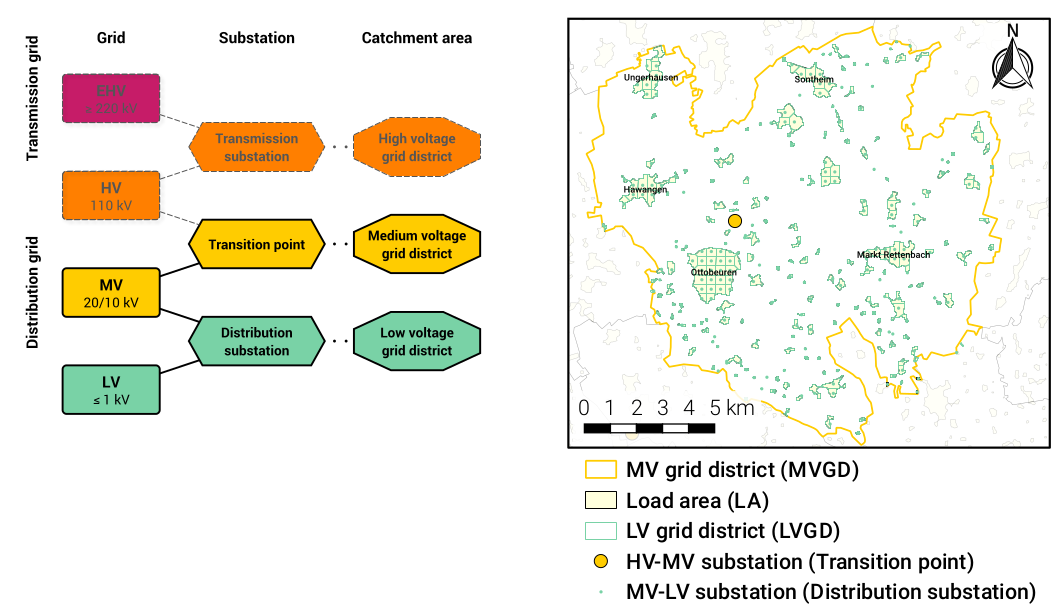
\includegraphics[width=0.45\textwidth]{Abb/sc_MVGD-structure1.png}
	\caption{Schema der Spannungsebenen und Beispiel MVGD}
\end{figure}

\begin{figure}[H]
	\label{EE-alloc}
	\caption{Tabelle zu EE-Allokation}
	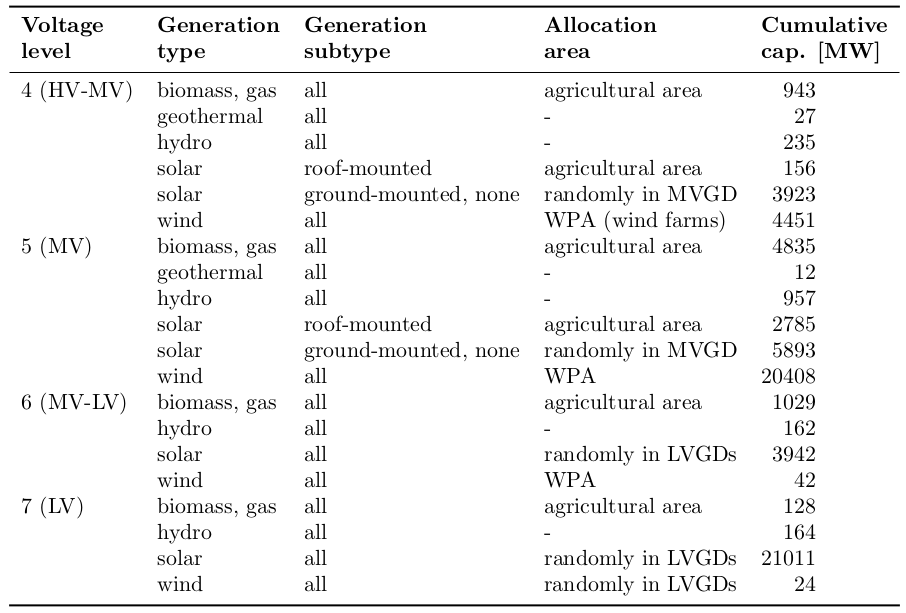
\includegraphics[width=0.45\textwidth]{Abb/sc_EE-alloc.png}

\end{figure}

\subsection{Alloc AEC + gen}
-->>Quelle Hülk

\subsection{Tutorials}
\subsubsection{eGo - Abschluss-Workshop 2018}
\url{https://nbviewer.jupyter.org/gist/wolfbunke/7659fbc22b9d72f0cda8dc544d1f537e}

Probleme mit directories...script start-platz?!\\
no module named pyproj (ist aber in d. site-packages vorhanden)
\subsubsection{eTraGo}
\url{https://nbviewer.jupyter.org/gist/ulfmueller/2c1fd6c4c29d606b313ab32bc0391dd2/eTraGo_Session_Workshop2018.ipynb}
\subsubsection{Ding0 - Workshop...}
\url{https://nbviewer.jupyter.org/gist/nesnoj/6ee605cd3494fa6e3e848385c4afbe19/dingo_session.ipynb}

Bsp. Notebook (von Projekt-website)
\url{https://nbviewer.jupyter.org/gist/nesnoj/6ee605cd3494fa6e3e848385c4afbe19/dingo_session.ipynb}

\subsubsection{oedb-examples}
\url{https://github.com/OpenEnergyPlatform/oedialect/blob/master/doc/example/oedialect_basic_example.ipynb}\\

\subsection{siehe auch}
\begin{itemize}
	\item US DoE
	\item[] \url{https://www.energy.gov/data/open-energy-data}
	\item weitere opensource Netzberechnungs-Variante
	\item[] \url{https://www.power.scigrid.de/}
	\item coastDat
	\item[] \url{https://www.coastdat.de/data/index.php.en}
	\item Erklärung zu Eigenschaften von json-Dateien
	\item[] \url{https://www.w3schools.com/js/js_json_intro.asp}
\end{itemize}

%\begin{thebibliography}{999}
%
%	\bibitem{lamport94}
%	Leslie Lamport,
%	\emph{\LaTeX: A Document Preparation System}.
%	Addison Wesley, Massachusetts,
%	2nd Edition,
%	1994.
%
%\end{thebibliography}
\bibliographystyle{acm}
\bibliography{/home/dafu/Schreibtisch/IEE/HA/IEE_ref.bib}
%\bibliographystyle{/home/dafu/Schreibtisch/num_methods/assignments/din1505/alphadin_lat_neu.bst}
%\bibliographystyle{plain}

\newpage
\appendix
\pagenumbering{Roman}
%\section{Python script: \\Newton-Raphson Method}\label{app-code}
%%\inputminted{python}{Gauß+Jac.py}
%\begin{minted}{Python}
%
%\end{minted}



%%%
%%% end main document
%%%
%%%%%%%%%%%%%%%%%%%%%%%%%%%%%%%%%%%%%%%%%%%%%%%%%%%%%%%%%%%%%%%%%%%%%%%%%%%%%%%%

% \appendix  %% include it, if something (bibliography, index, ...) follows below

%%%%%%%%%%%%%%%%%%%%%%%%%%%%%%%%%%%%%%%%%%%%%%%%%%%%%%%%%%%%%%%%%%%%%%%%%%%%%%%%
%%%
%%% bibliography
%%%
%%% available styles: abbrv, acm, alpha, apalike, ieeetr, plain, siam, unsrt
%%%
% \bibliographystyle{plain}

%%% name of the bibliography file without .bib
%%% e.g.: literatur.bib -> \bibliography{literatur}
% \bibliography{FIXXME}

\end{document}
%%% }}}
%%% END OF FILE
%%%%%%%%%%%%%%%%%%%%%%%%%%%%%%%%%%%%%%%%%%%%%%%%%%%%%%%%%%%%%%%%%%%%%%%%%%%%%%%%
%%% Notice!
%%% This file uses the outline-mode of emacs and the foldmethod of Vim.
%%% Press 'zi' to unfold the file in Vim.
%%% See ':help folding' for more information.
%%%%%%%%%%%%%%%%%%%%%%%%%%%%%%%%%%%%%%%%%%%%%%%%%%%%%%%%%%%%%%%%%%%%%%%%%%%%%%%%
%% Local Variables:
%% mode: outline-minor
%% OPToutline-regexp: "%% .*"
%% OPTeval: (hide-body)
%% emerge-set-combine-versions-template: "%a\n%b\n"
%% End:
%% vim:foldmethod=marker
